\section[Photonics RC with frequency-multiplexed neurons]{Photonics reservoir computer with frequency-multiplexed neurons}

\begin{frame}{Motivations}
	\begin{itemize}
		\item Blablabla
		\item Coupling of the different frequencies
	\end{itemize}
\end{frame}

\begin{frame}[allowframebreaks]{Frequency coupling - phase modulator}
	Effect of a \emph{phase modulator} :
	\begin{equation}
		Ee^{-i\omega t} \underset{\Omega}{\rightarrow} Ee^{-i\omega t}e^{im\sin{\Omega t}}= \sum_{k=-\infty}^{\infty} E J_k(m) e^{-i(\omega+k\Omega)t}
	\end{equation}
	
	
	\begin{columns}
	\begin{column}{.5\textwidth}
		\begin{figure}
		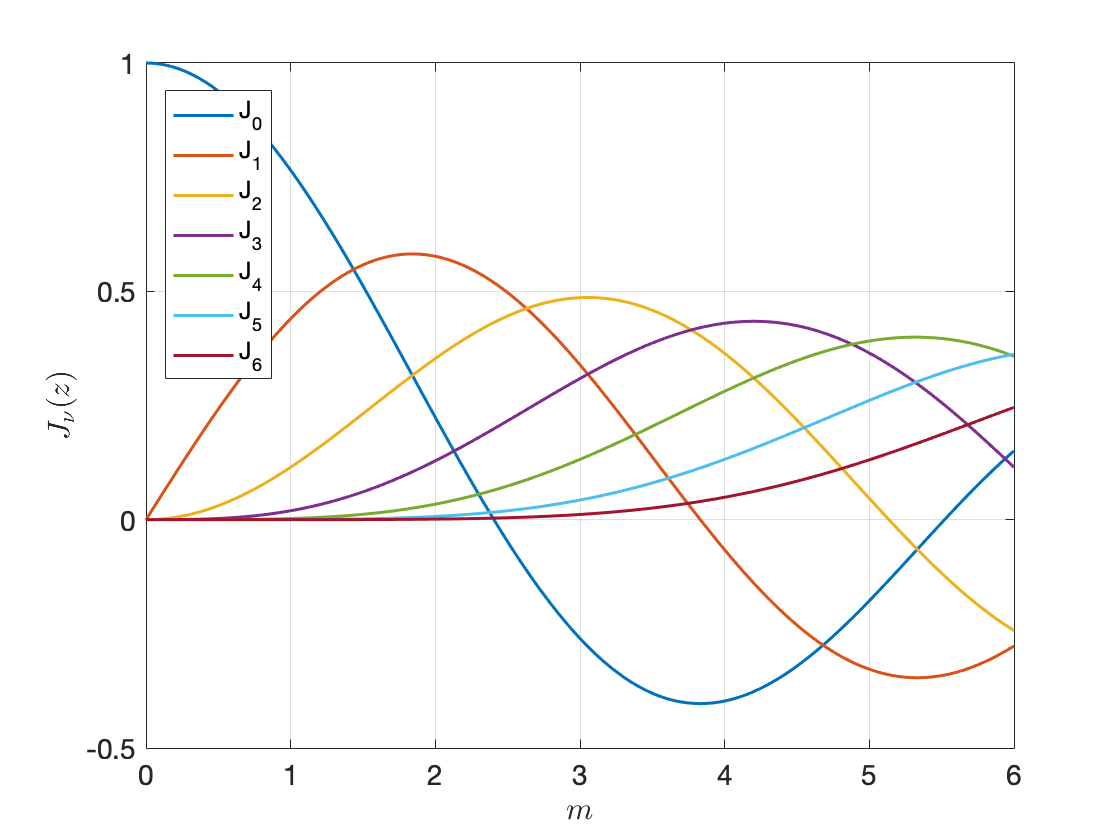
\includegraphics[width=\textwidth]{bessel.png}
		\end{figure}

	\end{column}
	\begin{column}{.48\textwidth}
			\begin{itemize}
			\item Experimentally, $m \leq 2$
			\item $J_k (m)$ decrease fast with $k$
			\item Series can be truncated
			\item \textbf{Finite number of frequencies can be coupled ($2N+1$)}
		\end{itemize}
	\end{column}%
	\hfill
	\end{columns}
	
	\begin{figure}
		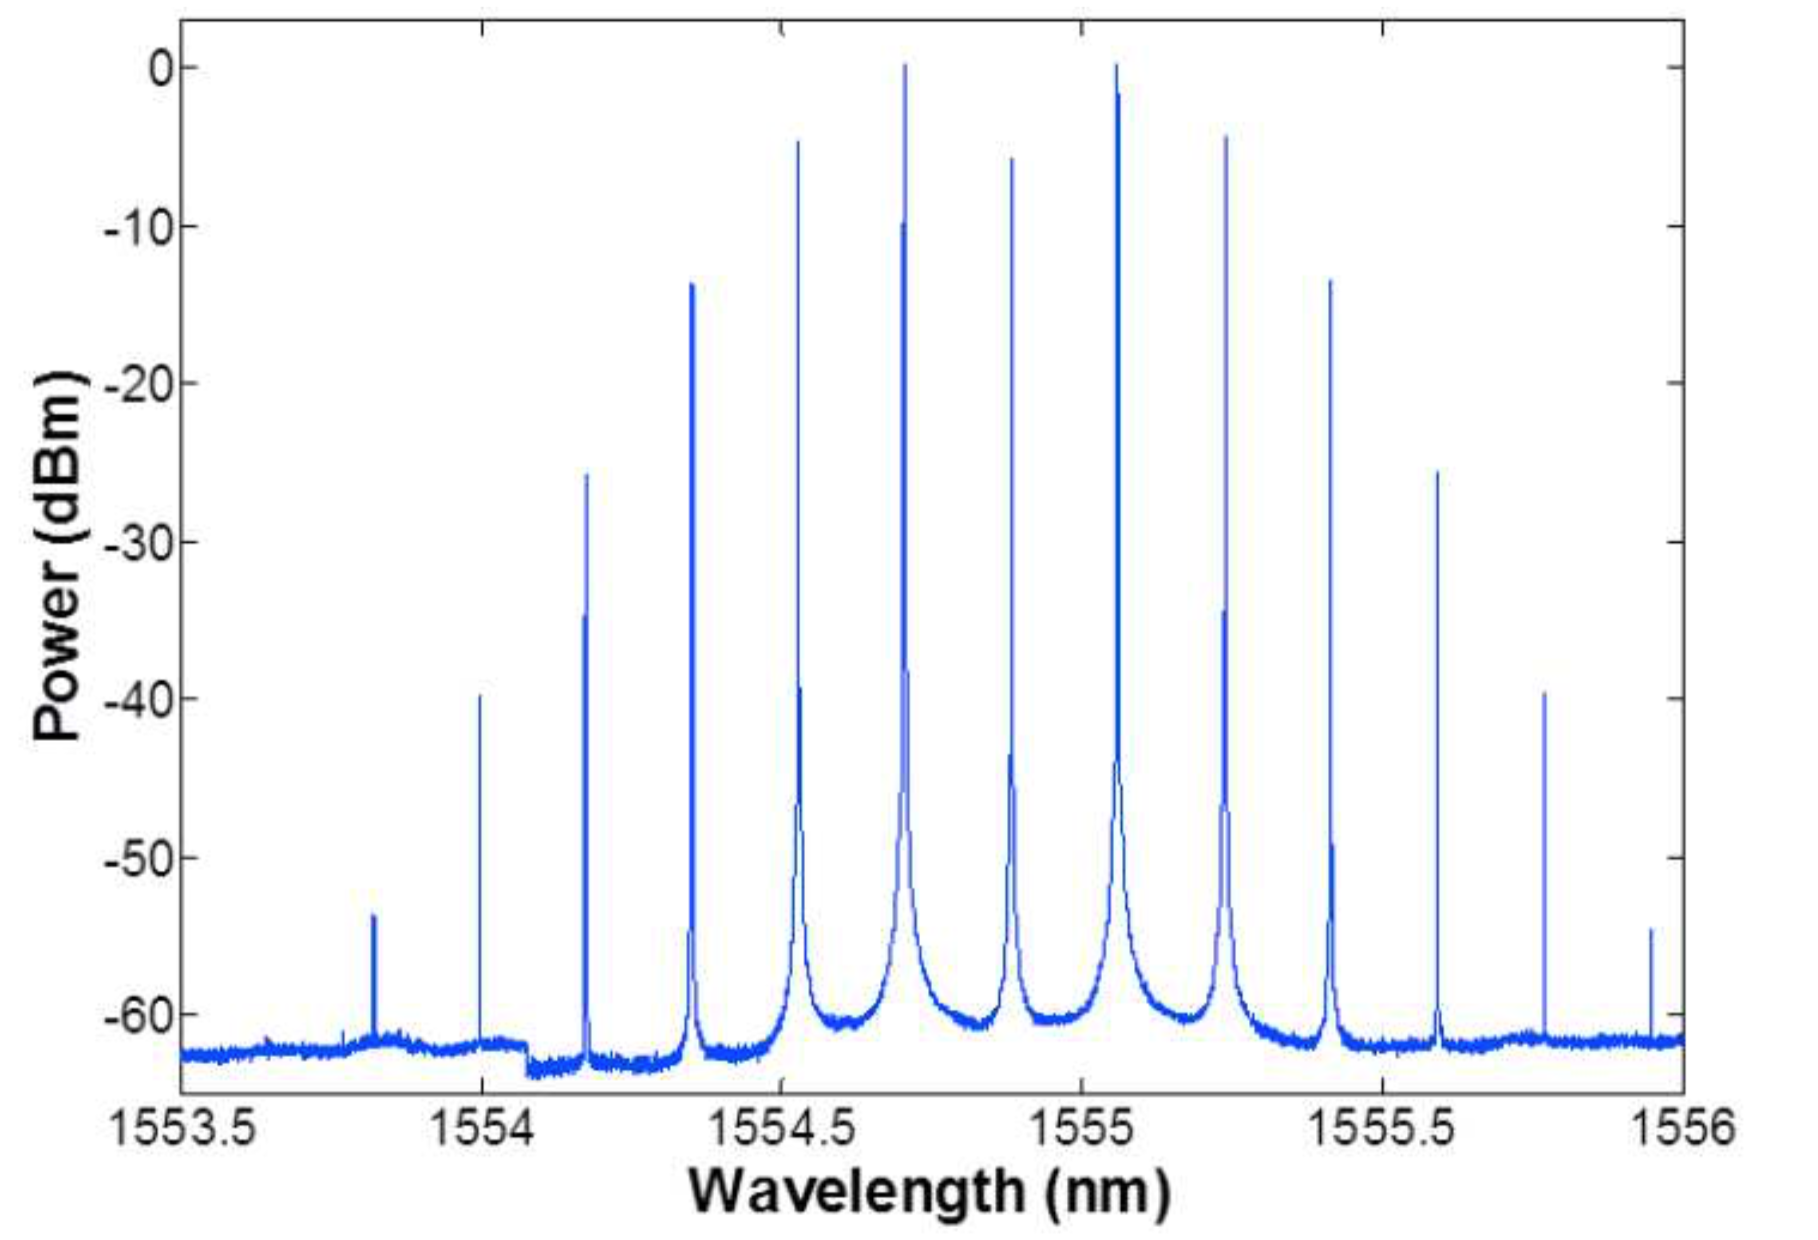
\includegraphics[width=.67\textwidth]{power-in-neurons.png}
		\caption{Spectrum inside the cavity. Only 13 frequencies are usable. \cite{AkroutAkram2016Pprc}}
	\end{figure}
	
\end{frame}

\begin{frame}{Mathematical Model}

	Definition of a neuron (complex electric field) :
	
	\begin{equation}
		x_k(t)=E_k e^{-i(\omega+k \Omega)t},~ k \in [-N,N~]
	\end{equation}
	
	Dynamics of a neuron :
	
	\begin{equation}
		x_k(n+1)= \alpha e^{i\phi_k}\sum_{j=0}^{2N} J_{-N+k+j}(m) ~x_{j-N}(n) + \beta u(n)~ \delta_{k,0}
		\label{neuron_dynamics}
	\end{equation}
	
	RC Output :
	
	\begin{equation}
		y(n)=\sum_{i=-N}^{N} W_i ~|x_i(n)|^2
	\end{equation}
	
\end{frame}


\begin{frame}{Schematic principle}

	\begin{figure}
		\begin{columns}
			\column{0.8\linewidth}
			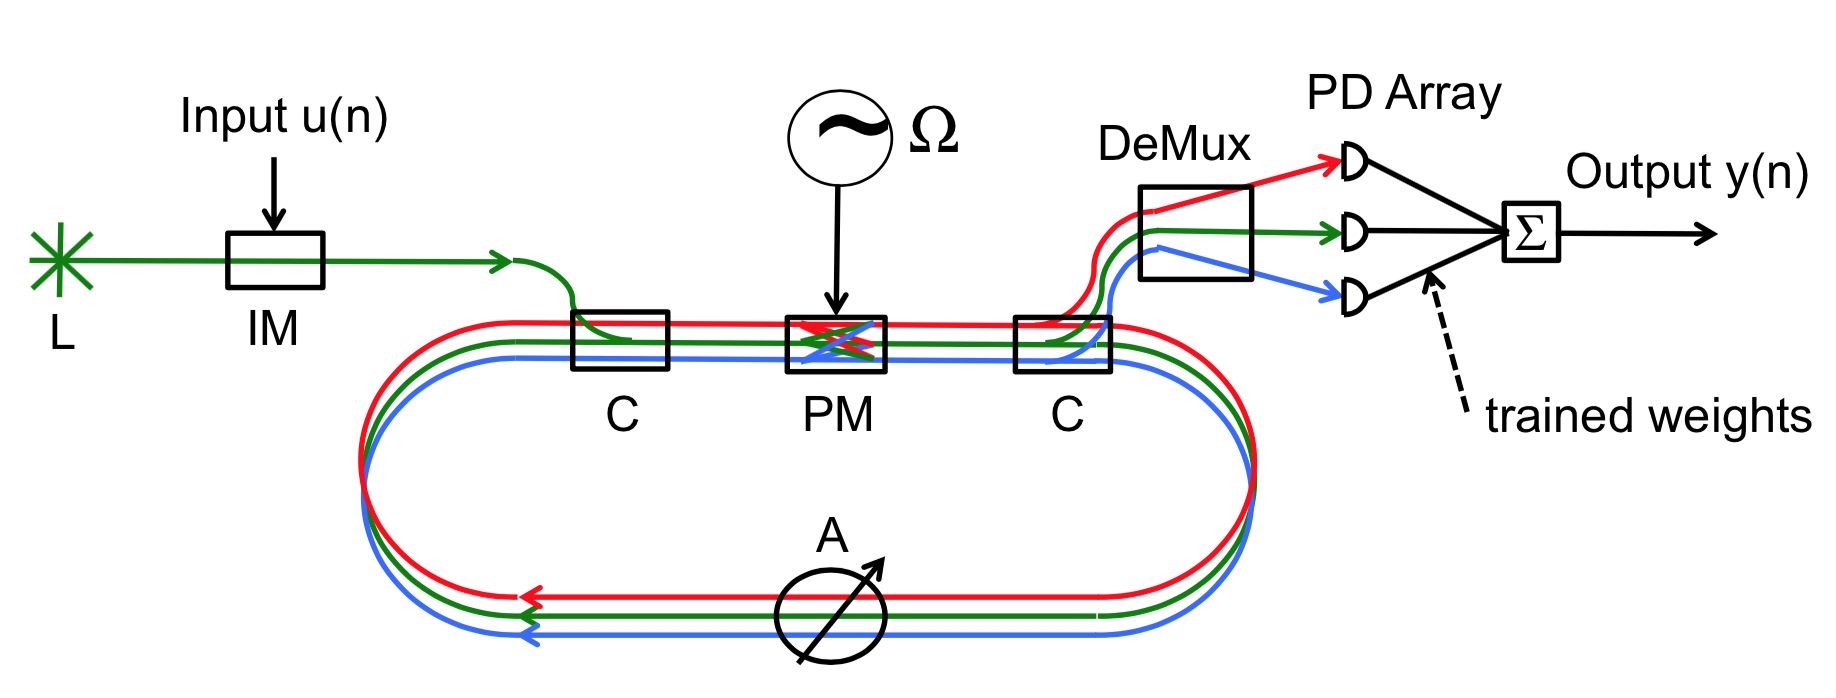
\includegraphics[width=\textwidth]{wdm_rc_principle.png}
			\column{0.2\linewidth}
			\caption{\cite{AkroutAkram2016Pprc}}
		\end{columns}
	\end{figure}
	
	\begin{columns}
		\begin{column}{0.5\textwidth}
			\begin{itemize}
				\item \textbf{One} input frequency
				\item Amplitude modulation : input data $u(n)$
				\item Frequency coupling in PM $\Omega$
			\end{itemize}
		\end{column}
		\begin{column}{0.5\textwidth}
			\begin{itemize}
				\item Nonlinearity in \emph{Readout PD} : $|x_k(n)|^2$
				\item \textit{Machine Learning} : \\output weights $W_i$
			\end{itemize}
		\end{column}
	\end{columns}
\end{frame}

\begin{frame}[allowframebreaks]{Main issues}
	\begin{itemize}
		\item $\phi_k$ (in Eq. \ref{neuron_dynamics}) should be a constant for each neuron\\ $\Longrightarrow$ \alert{Feedback loop regulation} of the optical cavity
		\item High losses induced by intra-cavity PM
		\item Intra-cavity amplification : EDFA
	\end{itemize}
\end{frame}
